% This is samplepaper.tex, a sample chapter demonstrating the
% LLNCS macro package for Springer Computer Science proceedings;
% Version 2.20 of 2017/10/04
%
\documentclass[runningheads]{llncs}
%
\usepackage{listings}
\usepackage{graphicx}
\usepackage{appendix}
\usepackage{amssymb}

%\usepackage{amsmath}
%\usepackage{amsthm}

\usepackage{stmaryrd}

\usepackage{leftidx}
\usepackage{mathtools}
\usepackage{paralist}
\usepackage{color}
\usepackage{enumitem}
%\usepackage{mathrsfs}
%\usepackage{dsfont}
%\usepackage{calligra}

%\usepackage{bm}
%\usepackage{nicefrac}
%\usepackage[draft]{minted}
\usepackage{tikz}
\usetikzlibrary{shapes,automata,positioning}
\usepackage[linesnumbered,ruled,noend]{algorithm2e}
\usepackage{graphicx}
% Used for displaying a sample figure. If possible, figure files should
% be included in EPS format.
%
% If you use the hyperref package, please uncomment the following line
% to display URLs in blue roman font according to Springer's eBook style:
% \renewcommand\UrlFont{\color{blue}\rmfamily}
\newcommand{\sesl}{\textsc{SESL}}
\newcommand{\compSpen}{\textsc{compSpen}}
\newcommand{\smack}{\textsc{SMACK}}
\newcommand{\boogie}{\textsc{Boogie}}
\newcommand{\llvm}{\textsc{LLVM}}


\newcommand{\zhilin}[1]{\color{magenta} {ZL: #1 :LZ} \color{black}}
\newcommand{\lx}[1]{\color{teal}{LX: #1 :XL} \color{black}} 
\newcommand{\zyt}[1]{\color{cyn} {YT: #1 :TY} \color{black}}
\begin{document}
%
\title{\textsc{SESL}: A Memory Safety Checker based on Separation Logic }
\subtitle{(Competition Contribution)}
%
%\titlerunning{Abbreviated paper title}
% If the paper title is too long for the running head, you can set
% an abbreviated paper title here
%
\author{Xie Li\inst{1,2} \and
Yutian Zhu\inst{1,2} \and
Zongxin Liu\inst{1,2} \and
Wanyun Su\inst{1}\and
\\
Zhilin Wu\inst{1}\and
Lijun Zhang\inst{1,3}}
%
\authorrunning{F. Author et al.}
% First names are abbreviated in the running head.
% If there are more than two authors, 'et al.' is used.
%
\institute{Institute of Software, China Academy of Sciences \and
University of China Academy of Sciences
\\
\and
Institute of Intelligent Software, Guangzhou\\
}


%
\maketitle              % typeset the header of the contribution
%
\begin{abstract}

SESL is a memory safety analyzer for C programs. It uses SMACK as the front end. Its back end relies on a symbolic execution engine which encodes path constraints as array separation logic (ASL) formulas. The ASL formulas are then solved by a separation logic solver called CompSpen. The salient feature of SESL is that it utilizes array separation logic to support byte-precise formal reasoning of memory safety issues.

\keywords{Memory safety \and Symbolic execution \and Separation logic.}
\end{abstract}
%
%
%
\section{Overview}
\textsc{SESL} is a static memory safety analyzer for C programs. 
The basic methodology are inherited from the symbolic execution based on separation logic (SL)\cite{DBLP:conf/aplas/BerdineCO05} and we use ASL to symbolically represent the a set of states. 
Compared to the original SL \cite{DBLP:conf/lics/Reynolds02} [\lx{add later variants}], ASL compacts a sequence of uninitialized points-to predicates into a single predicate \texttt{blk(x,y)}, indicating the heap is initialized from address \texttt{x} to \texttt{y-1}. With this succinctness and theoretical results of [\lx{ASL solving paper}], \textsc{SESL} can deal with analysis and checking efficiently.
The main contribution of this tool is the implementation of our symbolic execution engine based on ASL.
With the help of existing frontend tool \textsc{SMACK}\cite{DBLP:conf/cav/RakamaricE14}, we implemented a low level semantic of intermediate representation which supports byte-level manipulation of heap data. The algorithm of falsification utilizes  the result of symbolic execution for later feasibility checking and error analysis using our ASL solver \textsc{CompSpen}[\lx{CompSpen paper or website}]. 

The workflow of symbolic execution in \textsc{SESL} is stated as follows. 
\begin{enumerate}
\item Construct a control flow graph (CFG) $\mathcal{G} = (V, E)$ after parsing and analyzing the input source code, where $V$ and $E$ are the finite set of states and edges. Each state can be regarded as a basic block.
\item Sample out a set $S$ of paths $\pi$ of $\mathcal{G}$. The finiteness of $S$ is guranteed by restricting the maximum number that a state appears on one path. 
\item For each path in $S$,  do the symbolic execution and insert the corresponding ASL formula at each program point. The initial configuration is abstracted by initial formula $\langle true| emp\rangle$ and executions are conducted with rules we implemented, which will alter the formula with respect to the semantic of program. If errornous behavior like double-free and invalid-dereference appears, the execution ends the path.

\item After the execution $\pi$, the feasibility of the path and property violation checking will be encoded into an ASL formula as verification condition (VC). If the path is feasible and errors are found violating input properties, the tool find a violation path and stop to output. If no error is found for all the paths, an unknown result will be returned.
\end{enumerate}

Several techniques are applied to improve performance and maintain the accuracy. On the aspect of checking, the tool only checking feasibility for program points that may make the constraints loose. Besides, to maintain the accuracy of the analysis. We use a byte-level implementation of syntactic ASL library which bytifies spatial predicates only when needed. With the information obtain by preset analysis, the memory region will be properly splitted for pointer arithmetic. Regarding the execution process, the formula will bytify the corresponding part of spatial predicate lazily to make the representation as simple as possible. The ASL library also provides interface to translate the syntactic formula into data structure used for solving.

\section{Architecture}


The architecture framework of our tool is shown in figure~\ref{fig1}. Technically, our front end and back end are all implemented in the manner of LLVM passes in language C++. In this section we will discuss our front end and back end in detail.  

\begin{figure}
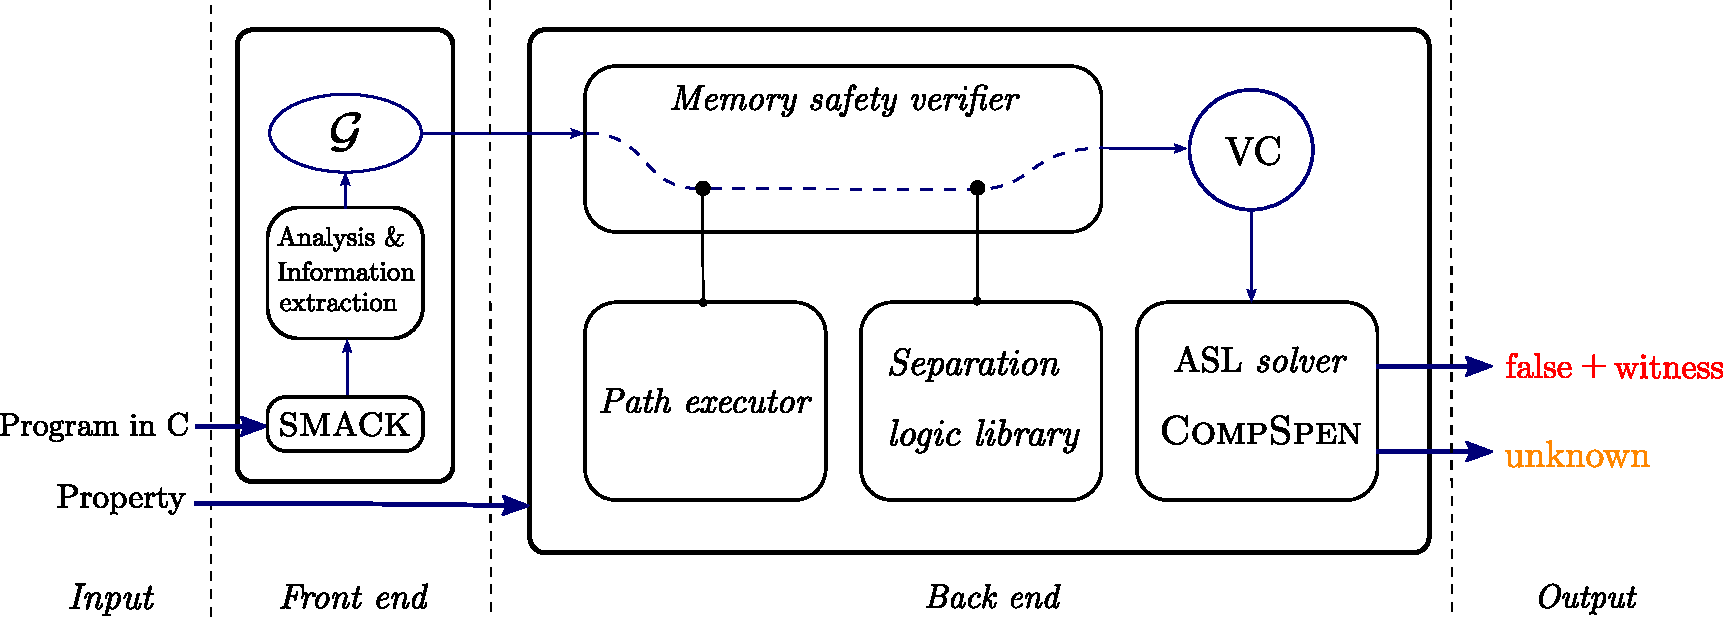
\includegraphics[width=\textwidth]{svcomp.pdf}
\caption{Architecture framework of \textsc{SESL}} \label{fig1}
\end{figure}

\subsection{Front end} The front end of \textsc{SESL} is built on the existing tool \textsc{SMACK}, which translates the source code into Boogie intermediate representation (IR). The command-line interface first takes the input of user and converts source code to LLVM IR. 
Then after applying several LLVM optimization passes, LLVM IR will be translated into Boogie IR data structure.
During the translation we give a record of type information and global variable initialization which will be of use in later analysis. 
The front end will finally construct a CFG for each function with states representing basicblocks and edges stand for \texttt{goto} statements in the function. 



\subsection{Back end}
The back end of \textsc{SESL} is a symbolic execution engine based on separation logic. The engine takes the constructed CFG and property parameter as inputs and either give a property violating program path or gives a unknown output. The back end consists of four parts: memory safety verifier, separation logic library, path executor and separation logic solver.




\paragraph{Memory safety verfier} This component contains the basic structure of the symbolic execution algorithm, which connect the path sampling, path execution, ASL formula solving and result producing. \textsc{SESL} samples the program path in a limited methodology since the infinity of program paths in a CFG. The strong connected component(SCC) of CFG will be distinguished and within each SCC the tool samples one path with preset limit of maximum ocurrences of a state and depth of function callings.

\paragraph{Path executor} Path executor symbolically executes each path sampled and inserts  syntactic separation logic formulas at each program point. To auxillary the execution, several analysises are also implemented in the module such as constant propagation,  type and pointer analysis. During the execution of one path, these analysises can be used to determine possible violation of property, which can be regarded as a prunning technique for exhausting the symbolic execution graph.

\paragraph{Separation logic library and solver} Based on the implementation of program abstract syntax tree (AST) of \textsc{SMACK}, we implemented a syntax library for separation logic. The library gives a good support for establishment and manipulation of byte-level separation logic formula, especially when it encounters pointer arithmetic and byte-level operations. 
Our separation logic solver \textsc{CompSpen} is a key component which gives a decent support for execution engine of \textsc{SESL}. 


\section{Strengths and Weaknesses}

The strength of the \textsc{SESL} lies on the back end implemented. With the components stated above, \textsc{SESL} can do symbolic execution with simpler spatial predicate \texttt{blk(x, y)} which not only simplifies the representation on syntax but also improves the efficiency on solving. Despite the precise representation, the tool also  remains accuracy with our bytifying techniques. Another advantage of our tool is enabling the byte-level representation and manipulation of ASL, realized by our syntax library. With the benefit of ASL, it acts well with pointer arithmetic.
Besides  it is also implemented and tuned with respect to the semantic of C and standard library functions.

The drawback of \textsc{SESL} is the capability of the tool. Since the tool only carries an execution engine, it can now only conduct falsification of programs. The tool currently cannot give a over-approximation for loop behaviors and recursive function calls. To further specify the obstacles encountered when trying to give a proof of correctness, \textsc{SESL} finds it hard to deal with nondeterministic pointer arithmetic and heap behaviors without use of heavier methods such as abstract interpretation and model checking.


\section{Tool Setup and Configuration}

The competition submission is based on \textsc{SESL} version 1.0.4. The tool is open source, releases and usage can be found at 
\begin{center}

\texttt{https://spencerl-y.github.io/SESL/}
\end{center}

The installation instructions are clearly stated on the site. With the competition version of the tool, it is recommended to use the following command to analyze one single file:

\begin{center}

\texttt{
./sesl-svcomp.sh -bw 64 -t --add-line-info <input\_file>}
\end{center}

where \texttt{--add-line-info} will stabbed line information to the output and \texttt{-bw 64} indicates the architecture considered for the checking is 64bit machine.
\paragraph{Participation} \textsc{SESL} is attending the competition in the MemorySafety track of SV-COMP.


\section{Software Project}

\textsc{SESL} is a property of Institute of Software, China Academy of Sciences. The tool is maintained by Xie Li and is public available under an MIT license. 

Acknowledgement....



%
% ---- Bibliography ----
%
% BibTeX users should specify bibliography style 'splncs04'.
% References will then be sorted and formatted in the correct style.
%
\bibliographystyle{splncs04}
\bibliography{svcompBib}

\end{document}
